\documentclass[a4paper]{article}
\usepackage[utf8]{inputenc}
\usepackage{alphabeta}
\usepackage{graphicx}
\usepackage[section]{placeins}
\usepackage{float}
\usepackage{amsmath}
\usepackage{listings}
\usepackage[usenames,dvipsnames]{xcolor}
\usepackage{amsmath}
\usepackage{extarrows}
\usepackage{amssymb}
\usepackage{verbatim}
\usepackage{enumerate}
\usepackage{eurosym}
\usepackage{svg}
\usepackage{varwidth}
\usepackage{pdflscape}
\usepackage{multirow}

\definecolor{codegreen}{rgb}{0,0.6,0}
\definecolor{codegray}{rgb}{0.5,0.5,0.5}
\definecolor{codepurple}{rgb}{0.58,0,0.82}
\definecolor{backcolour}{rgb}{0.95,0.95,0.92}

\lstdefinestyle{mystyle}{
    backgroundcolor=\color{backcolour},   
    commentstyle=\color{codegreen},
    keywordstyle=\color{magenta},
    numberstyle=\tiny\color{codegray},
    stringstyle=\color{codepurple},
    basicstyle=\ttfamily\footnotesize,
    breakatwhitespace=false,         
    breaklines=true,                 
    captionpos=b,                    
    keepspaces=true,                 
    numbers=left,                    
    numbersep=5pt,                  
    showspaces=false,                
    showstringspaces=false,
    showtabs=false,                  
    tabsize=2
}

\lstset{style=mystyle}

\setlength{\parindent}{0pt}
\setlength{\parskip}{1em}
\setlength{\jot}{4mm}

\title{Συστήματα Μικροϋπολογιστών \\ 2η σειρά ασκήσεων}
\author{Νικόλαος Παγώνας, el18175 \\ Αναστάσιος Παπαζαφειρόπουλος, el18079}
\date{}

\begin{document}
\pagenumbering{gobble}
\maketitle

\subsection*{1η άσκηση}
Ο κώδικας για την 1η άσκηση, μαζί με τα κατάλληλα σχόλια, έχει συμπεριληφθεί στο αρχείο \texttt{ex1.8085}.

\subsection*{2η άσκηση}
Ο κώδικας για την 2η άσκηση, μαζί με τα κατάλληλα σχόλια, έχει συμπεριληφθεί στο αρχείο \texttt{ex2.8085}.

\subsection*{3η άσκηση}
Ο κώδικας για την 3η άσκηση, μαζί με τα κατάλληλα σχόλια, έχει συμπεριληφθεί στα αρχεία \texttt{ex3i.8085}, \texttt{ex3ii.8085} και \texttt{ex3iii.8085} αντίστοιχα.

\subsection*{4η άσκηση}
Ο κώδικας για την 4η άσκηση, μαζί με τα κατάλληλα σχόλια, έχει συμπεριληφθεί στο αρχείο \texttt{ex4.8085}.

\begin{minipage}{\textwidth}
\subsection*{5η άσκηση}

Η ζητούμενη μνήμη SRAM 256x4 bits έχει χώρο για 256 λέξεις μεγέθους 4 bits. Χωρίζουμε λοιπόν τη μνήμη σε 4 τμήματα μεγέθους 256 bits, ώστε η κάθε λέξη να μοιράζει από ένα bit σε καθένα από τα τέσσερα τμήματα. Ουσιαστικά, το κάθε τμήμα είναι ένας πίνακας με διαστάσεις $α$ και $β$ με $ α \cdot β = 256 $. Για να πετύχουμε τετραγωνικό σχήμα επιλέγουμε διαστάσεις 32x8. Η επιλογή γραμμής απαιτεί: $log_{2}32 = 5 $ bits οπότε για τον σκοπό αυτό χρησιμοποιούνται οι ακροδέκτες διευθύνσεων $Α_0-Α_2$ με πολυπλέκτες 8-σε-1. Αντίστοιχα, η επιλογή στήλης απαιτεί: $ log_{2}8 = 3 $ bits και για το σκοπό αυτό χρησιμοποιούνται οι ακροδέκτες διευθύνσεων $Α_3-Α_7$ με αποκωδικοποιητή 5-σε-32. Οι ακροδέκτες $D_0-D_3$ είναι οι ακροδέκτες εισόδου/εξόδου των 4 bit και τα σήματα $\overline{CS}$ και $\overline{RD}$ μέσω των αντίστοιχων ακροδεκτών επιτρέπουν ή αποτρέπουν τις λειτουργίες εγγραφής και ανάγνωσης. Τα τρία σήματα ελέγχου έχουν αρνητική πολικότητα, δηλαδή ενεργοποιούν τη λειτουργία τους, το καθένα, όταν είναι μηδέν. Το σήμα $\overline{CS}$ (αρνητικό ChipSelect) ενεργοποιεί ή αδρανοποιεί ολόκληρο το chip και προορίζεται για χρήση όταν φτιάχνουμε μια μεγάλη μνήμη από πολλά chips, για να επιλέγουμε σε ποιο chip απευθυνόμαστε κάθε φορά. Όταν $\overline{CS} $ = 0 (ενεργό chip), το σήμα $\overline{WE}$ (αρνητικό WriteEnable) ενεργοποιεί την εγγραφή ενώ το σήμα $\overline {RD}$ ενεργοποιεί την ανάγνωση. 

\end{minipage}

\begin{figure}[H]
	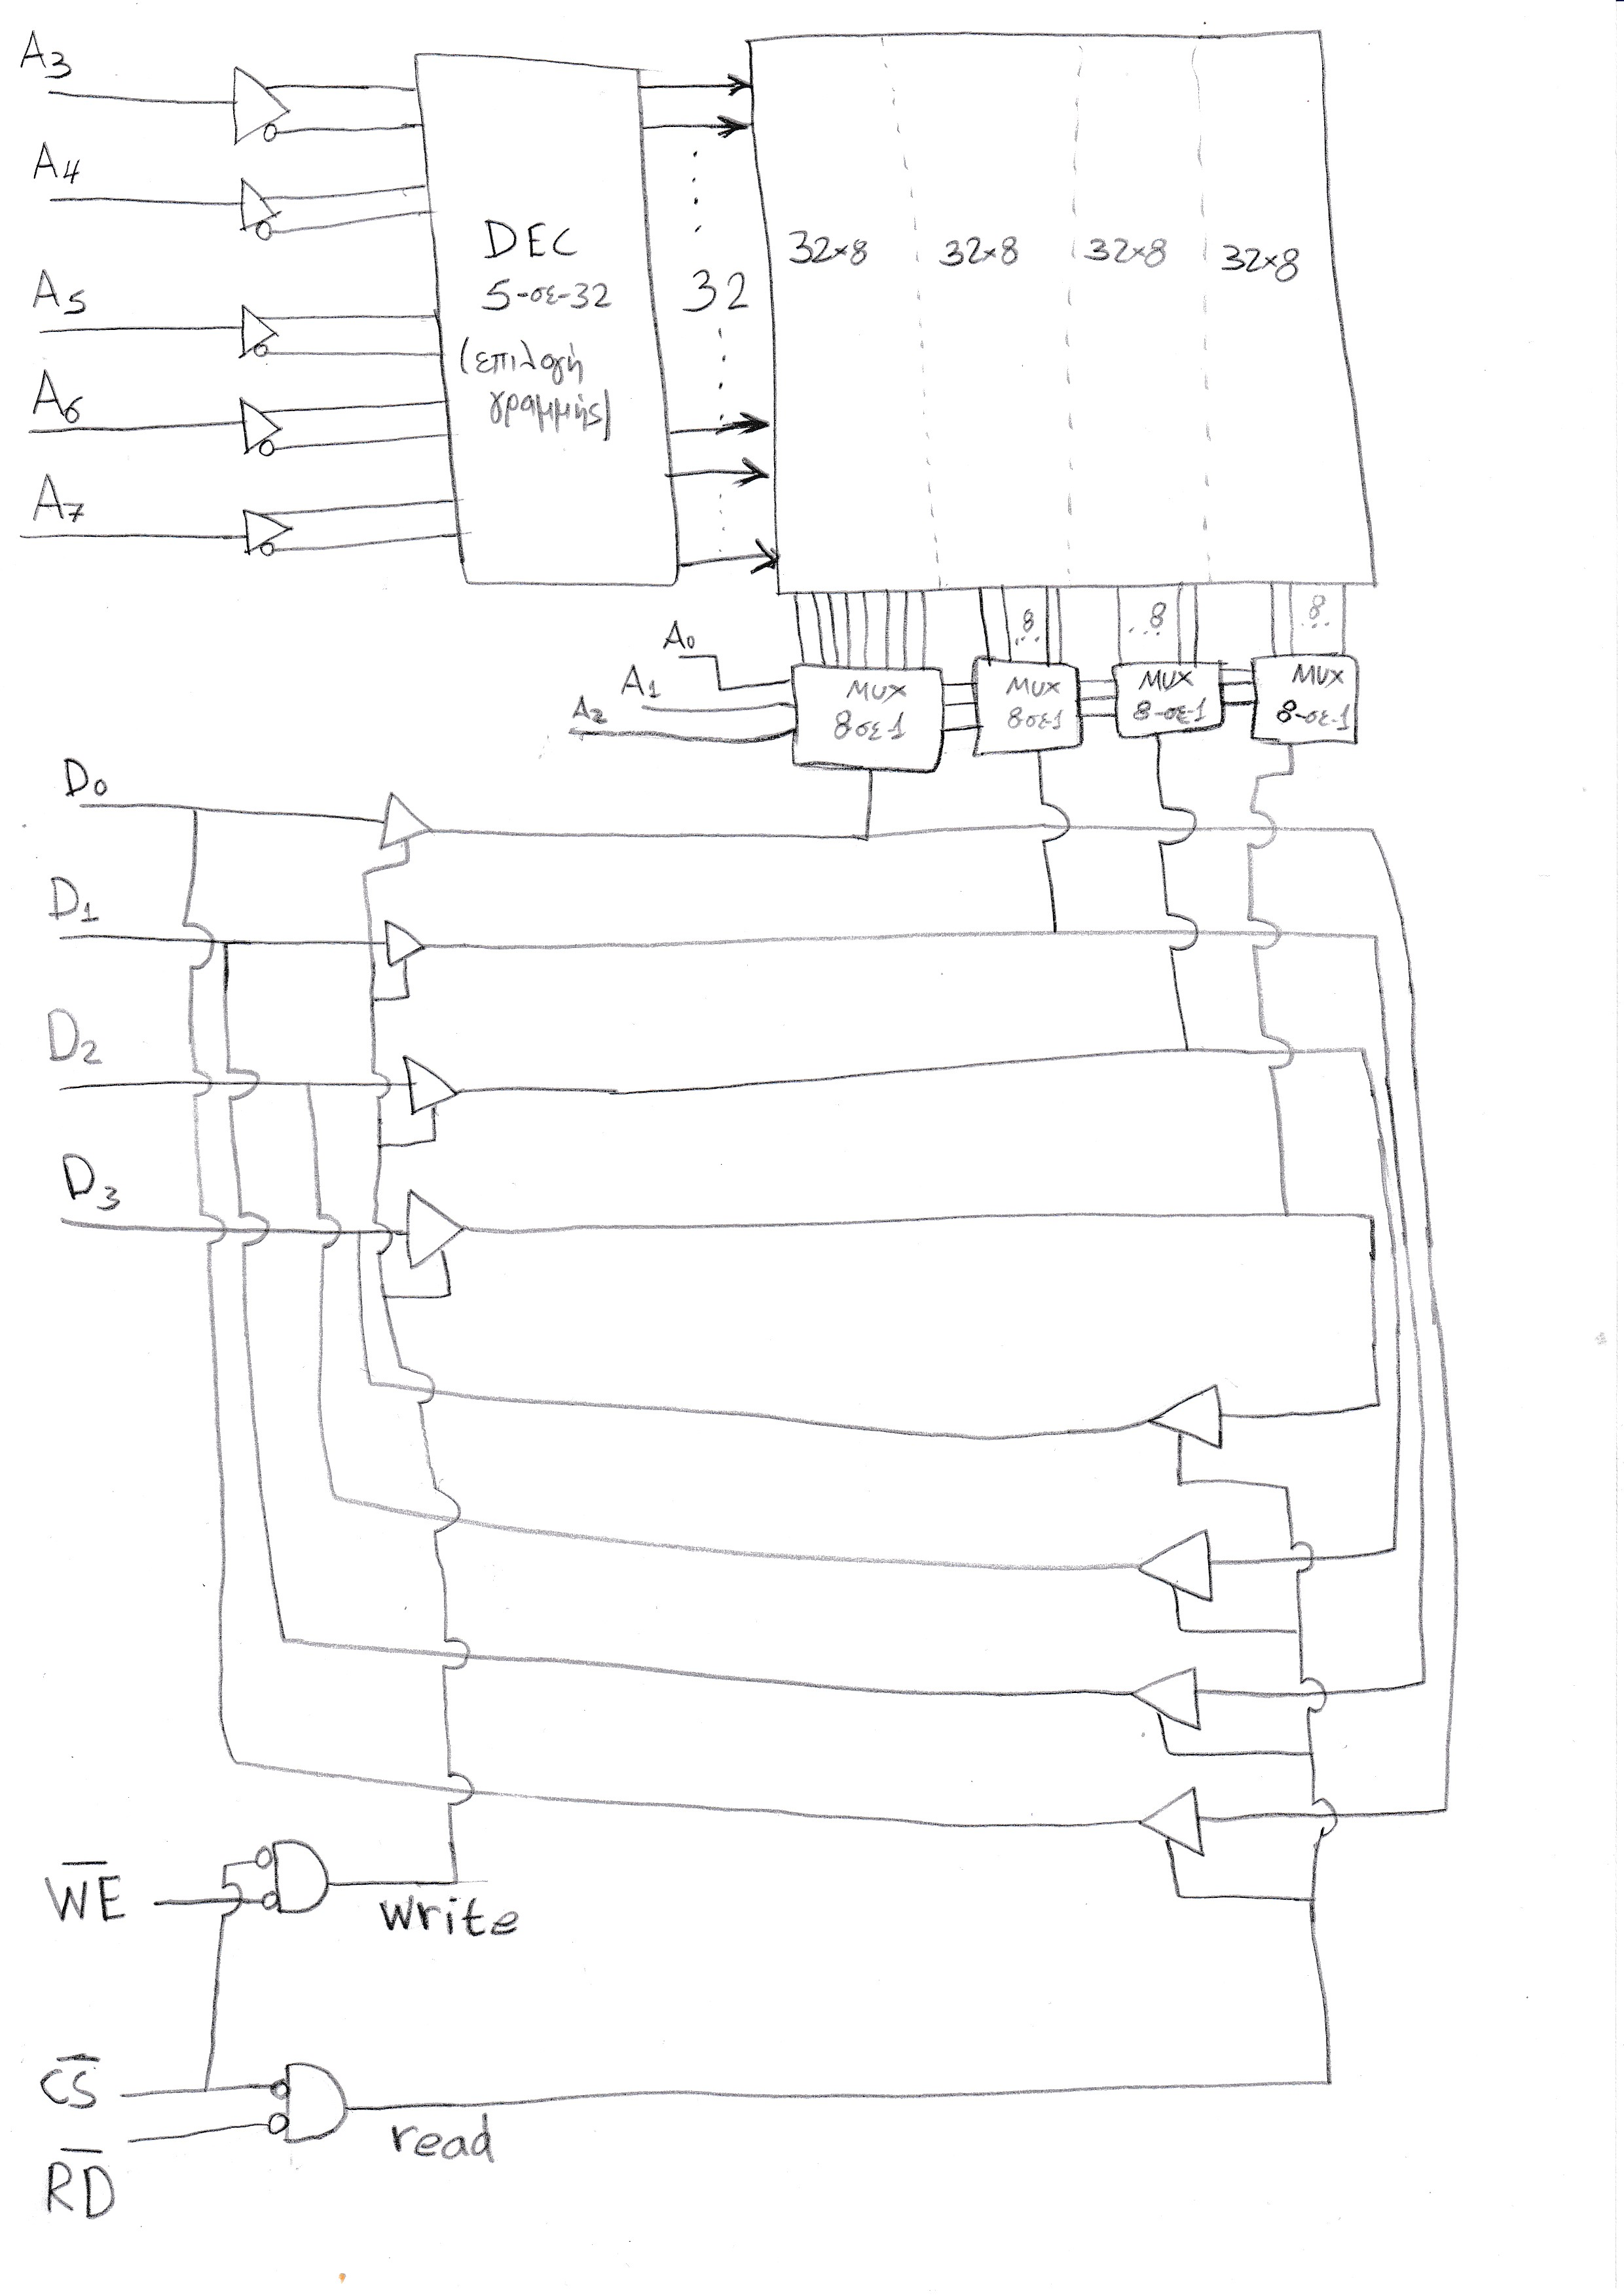
\includegraphics[width=\textwidth]{image1.jpg}
\end{figure}

\textbf{Ανάγνωση από τη μνήμη:}

Αρχικά εφαρμόζουμε στις γραμμές $Α_0-Α_7$ τη διεύθυνση από την οποία θέλουμε να διαβάσουμε. Το σήμα $\overline{CS}$ τίθεται στο λογικό 0, μέσω αρνητικού παλμού και σταματάει η απομόνωση εισόδου και εξόδου της μνήμης. Έρχεται αρνητικός παλμός στον ακροδέκτη $\overline{RD}$, ενώ στον $\overline{WE} $ έρχεται θετικός και ξενικάει η ανάγνωση από τη μνήμη αφού η έξοδος της αντίστοιχης πύλης AND (read) γίνεται 1, σε αντίθεση με την έξοδος της πύλης AND (write) που γίνεται 0. Οι ακροδέκτες $Α_3-Α_7$ καθορίζουν ποια γραμμή θα επιλεχθεί για την ανάγνωση των 4 bits, ενώ οι ακροδέκτες $Α_0-Α_2$ επιτρέπουν στα bit της επιλεγμένης στήλης να φτάσουν στις εξόδους των πολυπλεκτών. Στη συνέχεια το σύρμα read, οδηγείται στο enable των τρισταθών buffers που κοιτούν προς τα αριστερά και έτσι επιτρέπεται το πέρασμα πληροφορίας μέσα από τους $D_0, D_1, D_2, D_3$. Με αυτόν τον τρόπο η πληροφορία τους περνάει στην έξοδο των τρισταθών buffers με αποτέλεσμα
διαβάζουμε την επιθυμητή διεύθυνση. Οι τρισταθείς buffers που κοιτούν προς τα δεξιά τίθενται σε κατάσταση υψήλης αντίστασης. Έπειτα, τελειώνει ο αρνητικός παλμός $\overline{RD}$ και επανέρχεται το $\overline{CS}$ στο λογικό 1.


\textbf{Εγγραφή στη μνήμη:}

Αρχικά εφαρμόζουμε στις γραμμές $Α_0-Α_7$ τη διεύθυνση στην οποία θέλουμε να γράψουμε. Το σήμα $\overline{CS}$ τίθεται στο λογικό 0, μέσω αρνητικού παλμού και σταματάει η απομόνωση εισόδου και εξόδου της μνήμης. Έρχεται αρνητικός παλμός στον ακροδέκτη $\overline{WE}$, ενώ στον $\overline{RD}$ έρχεται θετικός και ξενικάει η εγγραφή στη μνήμη αφού η έξοδος της αντίστοιχης πύλης AND (write) γίνεται 1, σε αντίθεση με την έξοδος της πύλης AND (read) που γίνεται 0. Οι $Α_0-A_2$ προσδιορίζουν σε ποια στήλη από τις 8 να οδηγήσουν την είσοδο και οι $Α_3-Α_7$ σε ποια γραμμή θα γίνει η εγγραφή των 4 bits. Στη συνέχεια το σύρμα write, οδηγείται στο enable των τρισταθών buffers που κοιτούν προς τα δεξιά ελέγχοντας το πέρασμα πληροφορίας από τις εισόδους $D_0, D_1, D_2, D_3$ οι οποίες ενεργοποιούνται. Με αυτόν τον τρόπο η πληροφορία τους περνάει στην έξοδο των τρισταθών buffers και ανανεώνει το περιεχόμενο της κατάλληλης θέσης μνήμης η οποία έχει επιλεχθεί. Οι τρισταθείς buffers που κοιτούν προς τα αριστερά τίθενται σε κατάσταση υψήλης αντίστασης. Έπειτα, τελειώνει ο αρνητικός παλμός $\overline{WE}$ και επανέρχεται το $\overline{CS}$ στο λογικό 1.


\subsection*{6η άσκηση}

Ο χάρτης μνήμης που προκύπτει από τα δεδομένα της εκφώνησης είναι ο εξής: \\

\input{ex6table}

\begin{landscape}
\begin{figure}[H]
Υλοποίηση με αποκωδικοποιητή 3x8 και λογικές πύλες:
\begin{center}
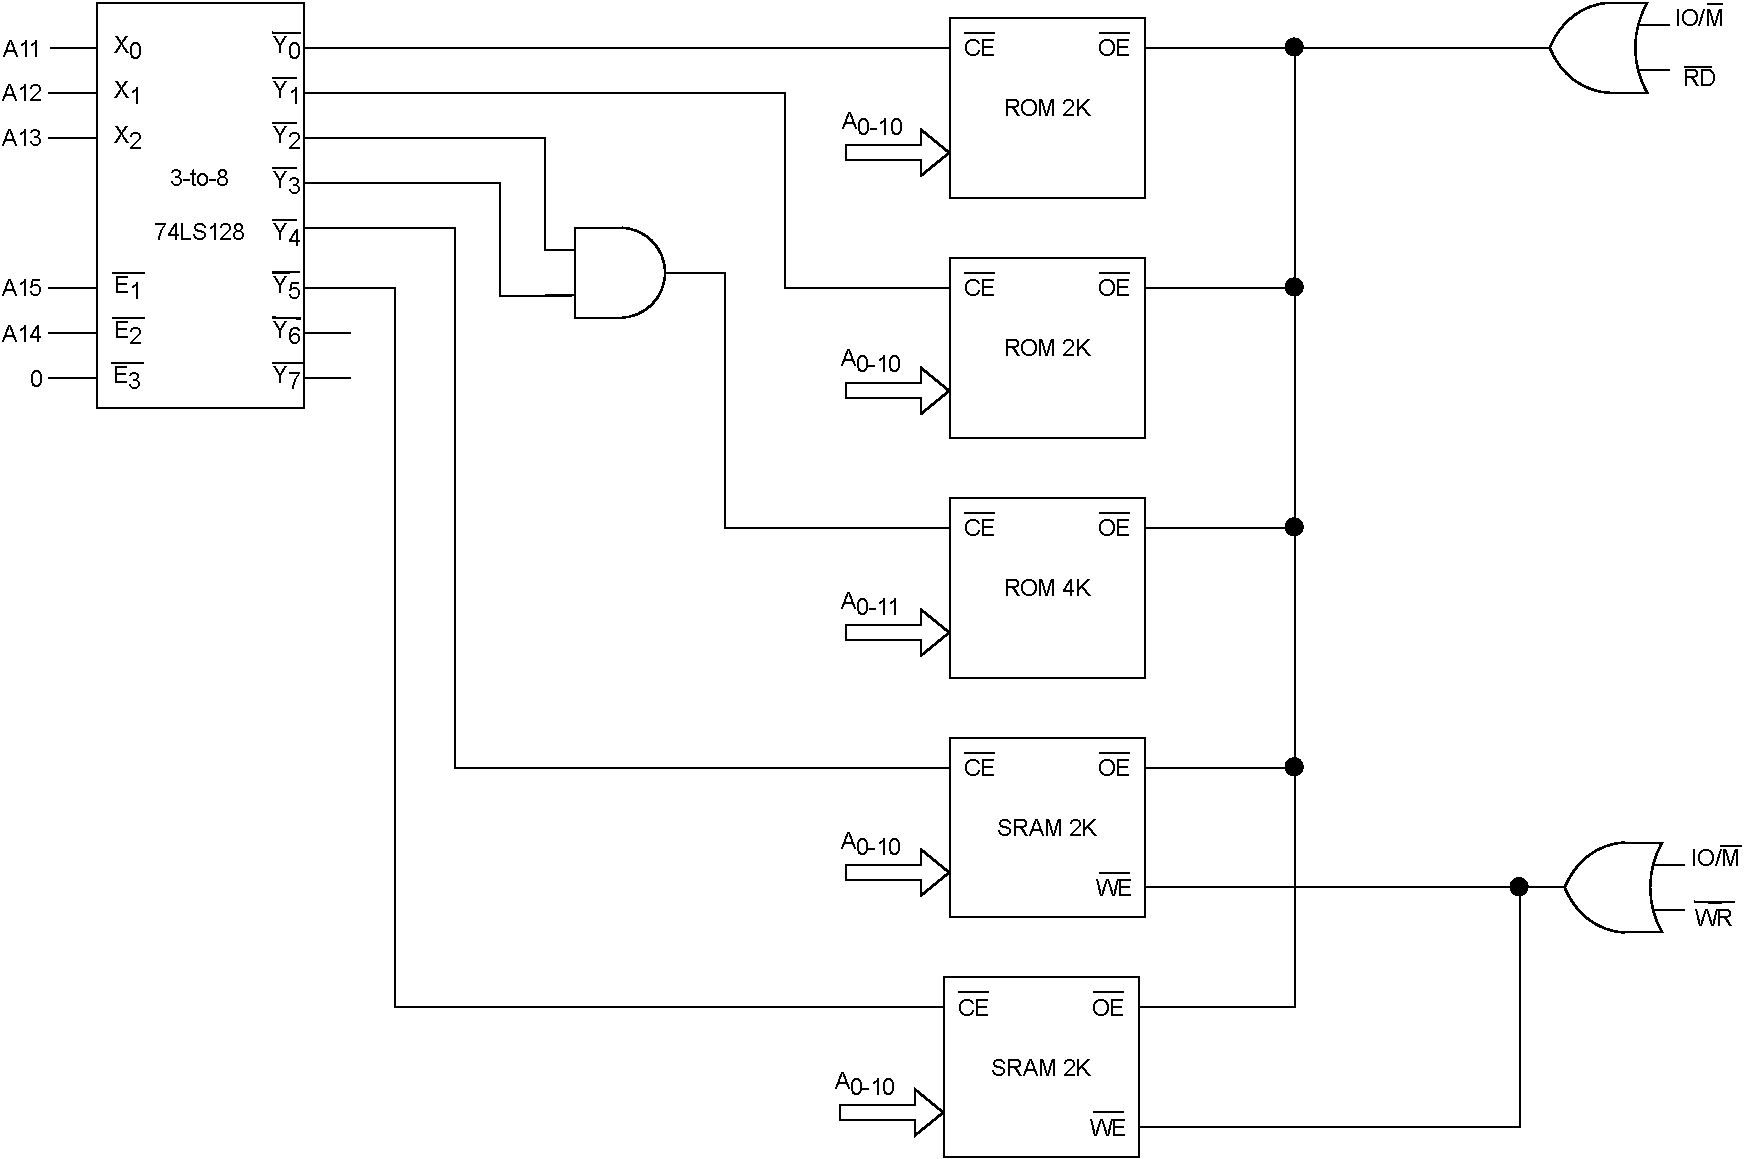
\includegraphics[width=1.3\textwidth]{ex6a.pdf}
\end{center}
\end{figure}
\end{landscape}

\begin{landscape}

\begin{figure}[H]
Υλοποίηση μόνο με λογικές πύλες (πλήρης αποκωδικοποίηση):
\begin{center}
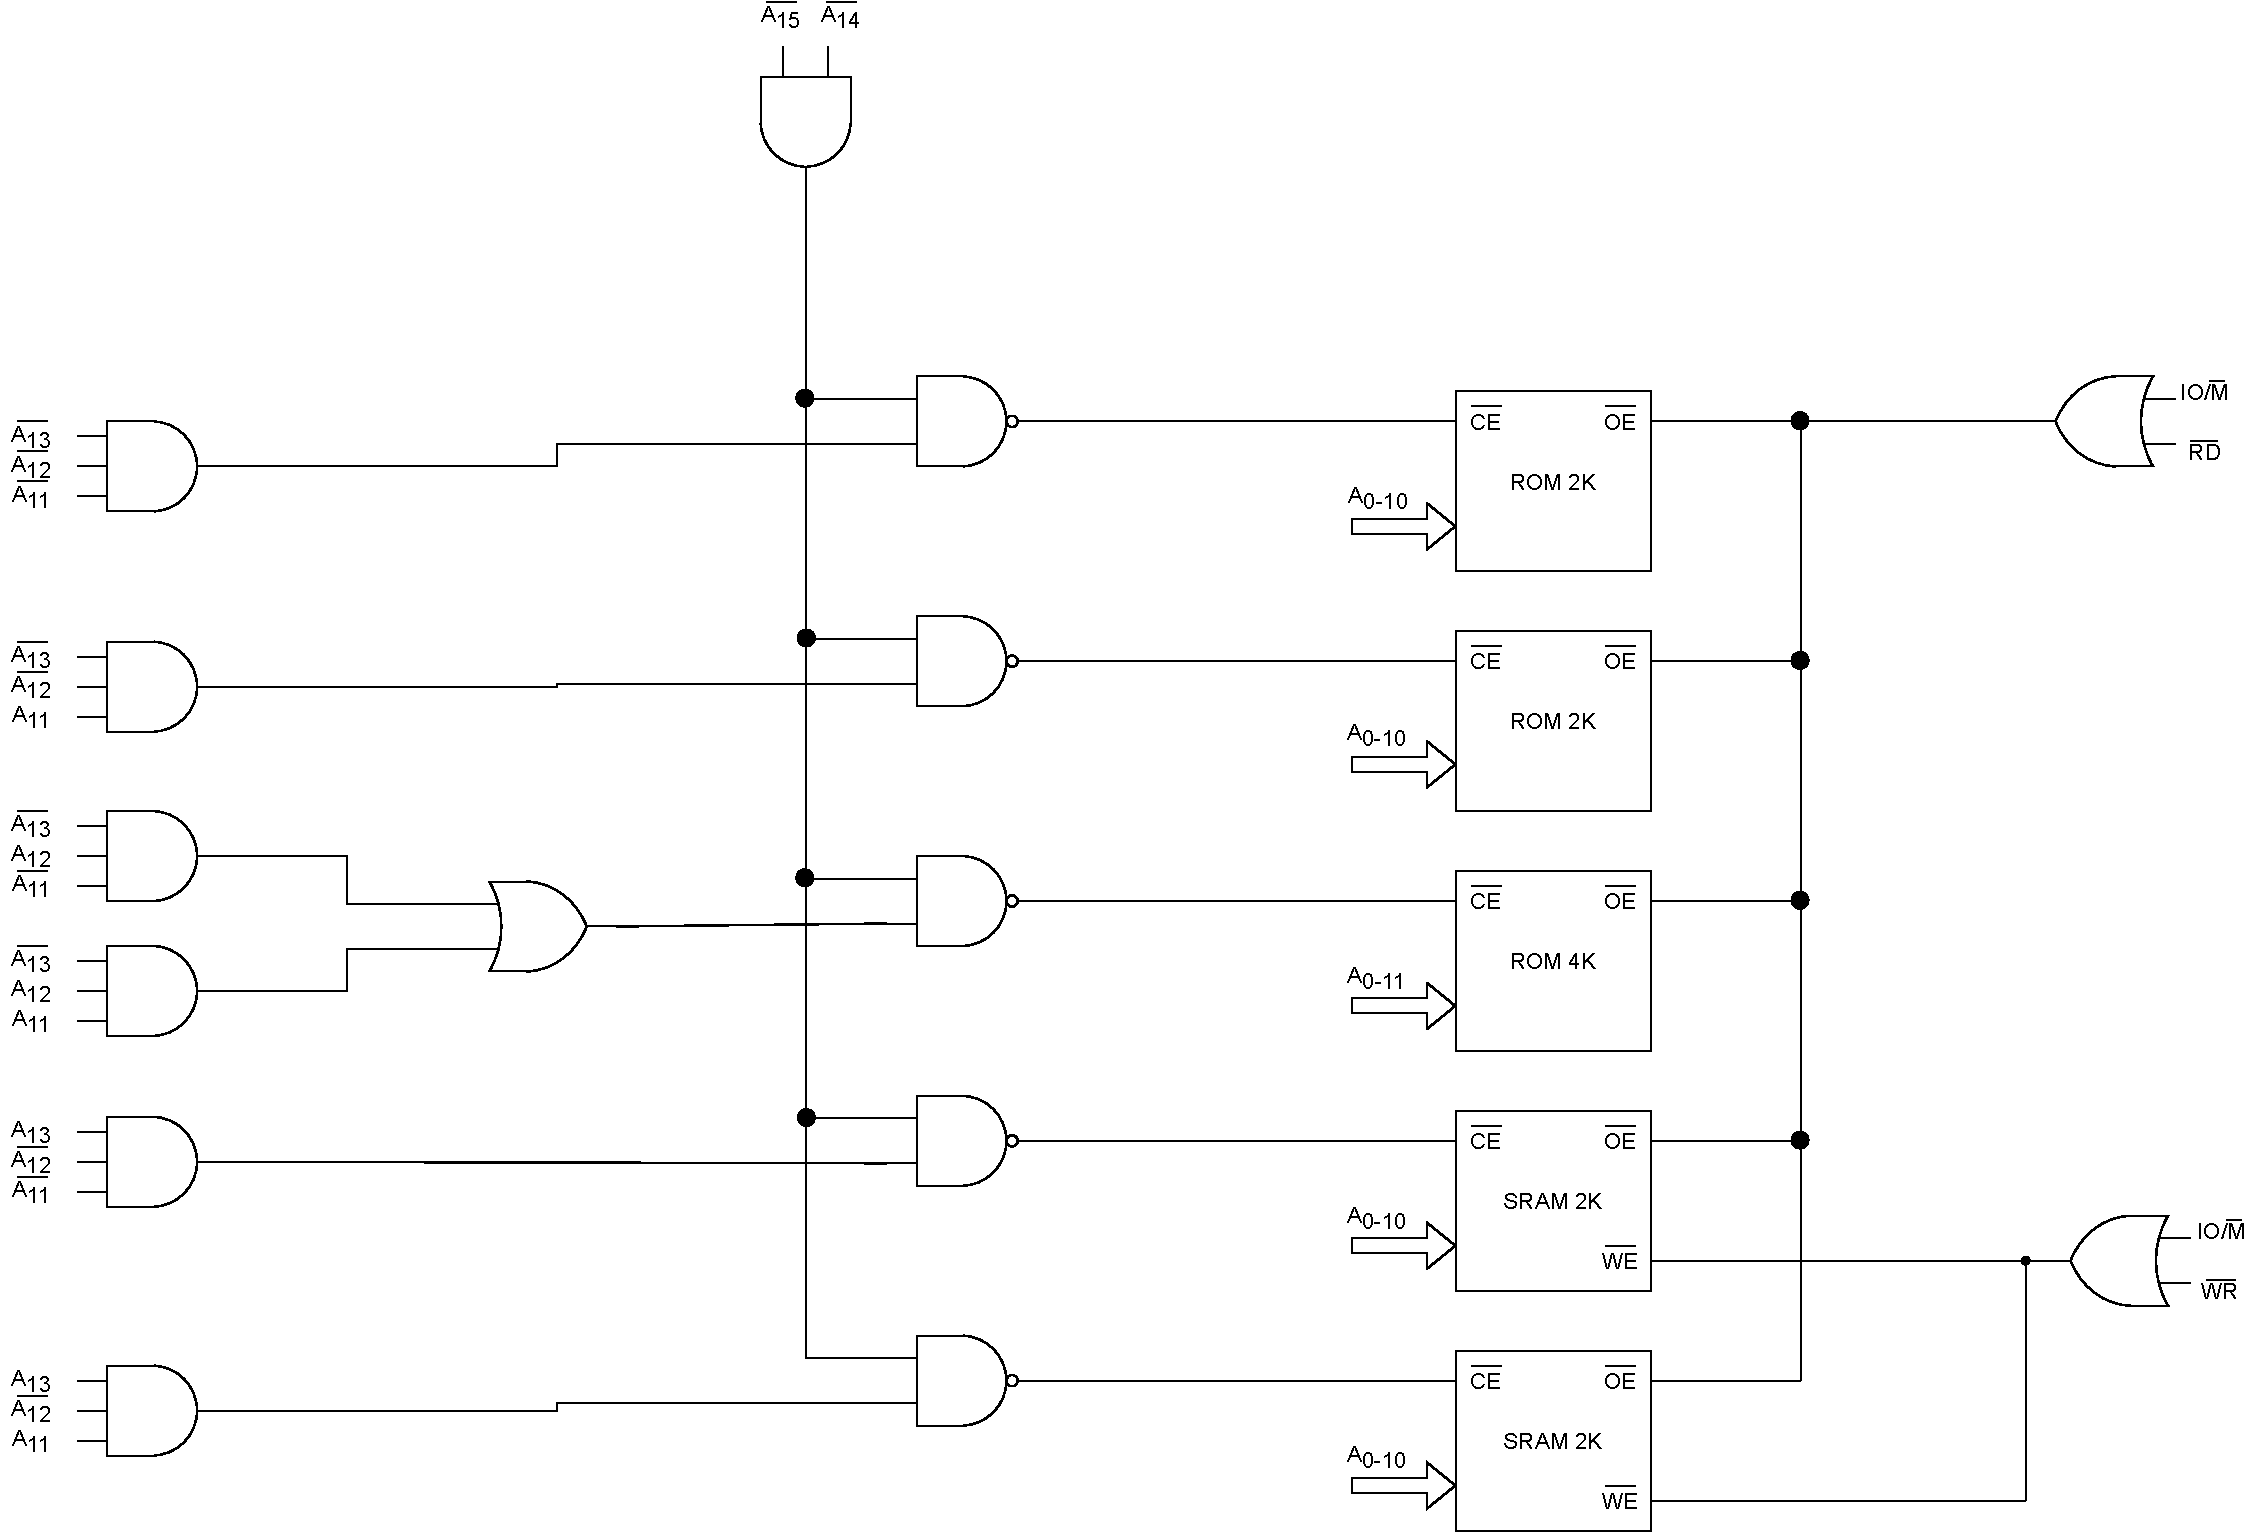
\includegraphics[width=1.3\textwidth]{ex6b.pdf}
\end{center}
\end{figure}
\end{landscape}

\subsection*{7η άσκηση}

\textbf{Χάρτης μνήμης:}

\begin{itemize}
\item 0000Η-2FFFΗ: ROM (12KΒ)
\item 3000Η-5FFFΗ: RAM (12KΒ)
\item 6000Η-6FFFΗ: ROM (4KΒ)
\item 7000Η: θύρα εξόδου (Memory map I/O)
\item 70Η: θύρα εισόδου (Standard I/O)
\end{itemize}

\begin{figure}[H]
	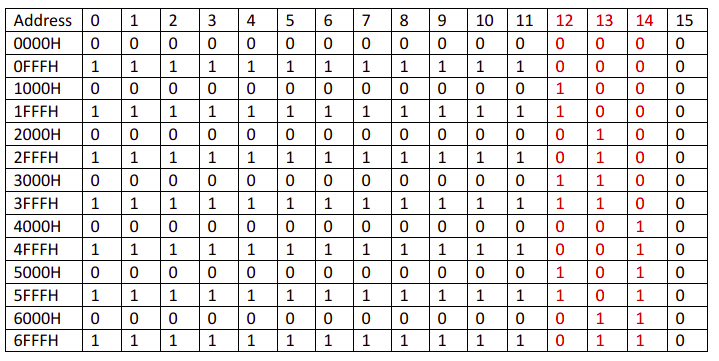
\includegraphics[width=\textwidth]{ex7table.png}
\end{figure}

Από τον παραπάνω πίνακα γίνεται φανερό ότι η διαφοροποίηση των θέσεων μνήμης που καταλαμβάνουν οι ROM, RAM γίνεται μέσω των θέσεων 12, 13, 14. Για αυτό, τα συγκεκριμένα bits χρησιμοποιούνται ως είσοδοι προκειμένου να επιλεχθεί το κατάλληλο ολοκληρωμένο μνήμης. Επιπρόσθετα, οι προδιαγραφές του προβλήματος ορίζουν την κάλυψη των θέσεων μνήμης με αλληλουχία ROM, RAM, ROM. Δηλαδή, η ενιαία μνήμη ROM που διαθέτουμε και έχει μέγεθος 16ΚΒ ίσο με το άθροισμα των μεγεθών των επιμέρους 4 ΚΒ και οι 3 RAM των 4 KB με συνολικό μέγεθος 12 KB θα πρέπει
να παρεμβάλλονται. Οπότε το πρόβλημα ανάγεται στο πως θα μπορέσουμε να διαχωρίσουμε τις διευθύνσεις που αντιστοιχούν σε κάθε κομμάτι της ROM.  Αναλυτικά έχουμε ότι λέξεις που αποθηκεύονται στην  ROM είναι σε πλήθος $16 K = 2^{14}$ και άρα απαιτούνται 14 bits ($Α_0-Α_{13}$) για την ορθή διευθυνσιοδότησή τους. 

Επίσης, οι λέξεις που αποθηκεύονται στις RAM 1, RAM 2, RAM 3 μεγέθους 4KB είναι σε πλήθος $4 K = 2^{12}$ και άρα απαιτούνται 12 bits ($Α_{0}-Α_{11}$) για την ορθή διευθυνσιοδότησή τους. 

Τα bits $Α_{12}, Α_{13}, Α_{14}$ χρησιμοποιούνται για την επιλογή του επιθυμητού ολοκληρωμένου (ROM, RAM1, RAM2 ή RAM3) καθώς ένας ή περισσότεροι συνδυασμοί αυτών προσδιορίζουν μοναδικά τις περιοχές μνήμης που αντιστοιχούν σε κάθε ολοκληρωμένο.
 
Πιο Συγκεκριμένα:

\begin{itemize}
\item ROM: $Α_{14}Α_{13}Α_{12} = 000$ και $Α_{14}Α_{13}Α_{12} = 001$ και $Α_{14}Α_{13}Α_{12} = 010$ και $Α_{14}Α_{13}Α_{12} = 110$
\item RAM 1: $Α_{14}Α_{13}Α_{12} = 011$
\item RAM 2: $Α_{14}Α_{13}Α_{12} = 100$
\item RAM 3: $Α_{14}Α_{13}Α_{12} = 101$
\end{itemize}

Η μνήμη ROM λαμβάνει τα bits $Α_{0}-Α_{11}$ από το address bus ενώ το bit $Α_{12}$ από την έξοδο της πύλης XOR και το $Α_{13}$ αυτούσιο όπως φαίνεται στο παρακάτω σχήμα. Έτσι τα bits $A_{12}$ και  $A_{13}$ μετατρέπουν τις διευθύνσεις του χάρτη μνήμης που αντιστοιχούν σε θέσεις της μνήμης ROM που δεν είναι στο πρώτο τμήμα της (0000Η-2FFFH) σε συνεχόμενες θέσεις εσωτερικά στο ολοκληρωμένο. Τέλος, για την επίτρεψη του latch της θύρας εξόδου 7000Η χρησιμοποιείται πύλη AND με 16 εισόδους (γιατί είναι memory map I/O), ενώ για την επίτρεψη του latch εισόδου χρησιμοποιείται το  $\overline{Y_7}$ (αφού είναι από το standard I/O) που δεν χρησιμοποιείται κάπου αλλού.

\begin{figure}[H]
	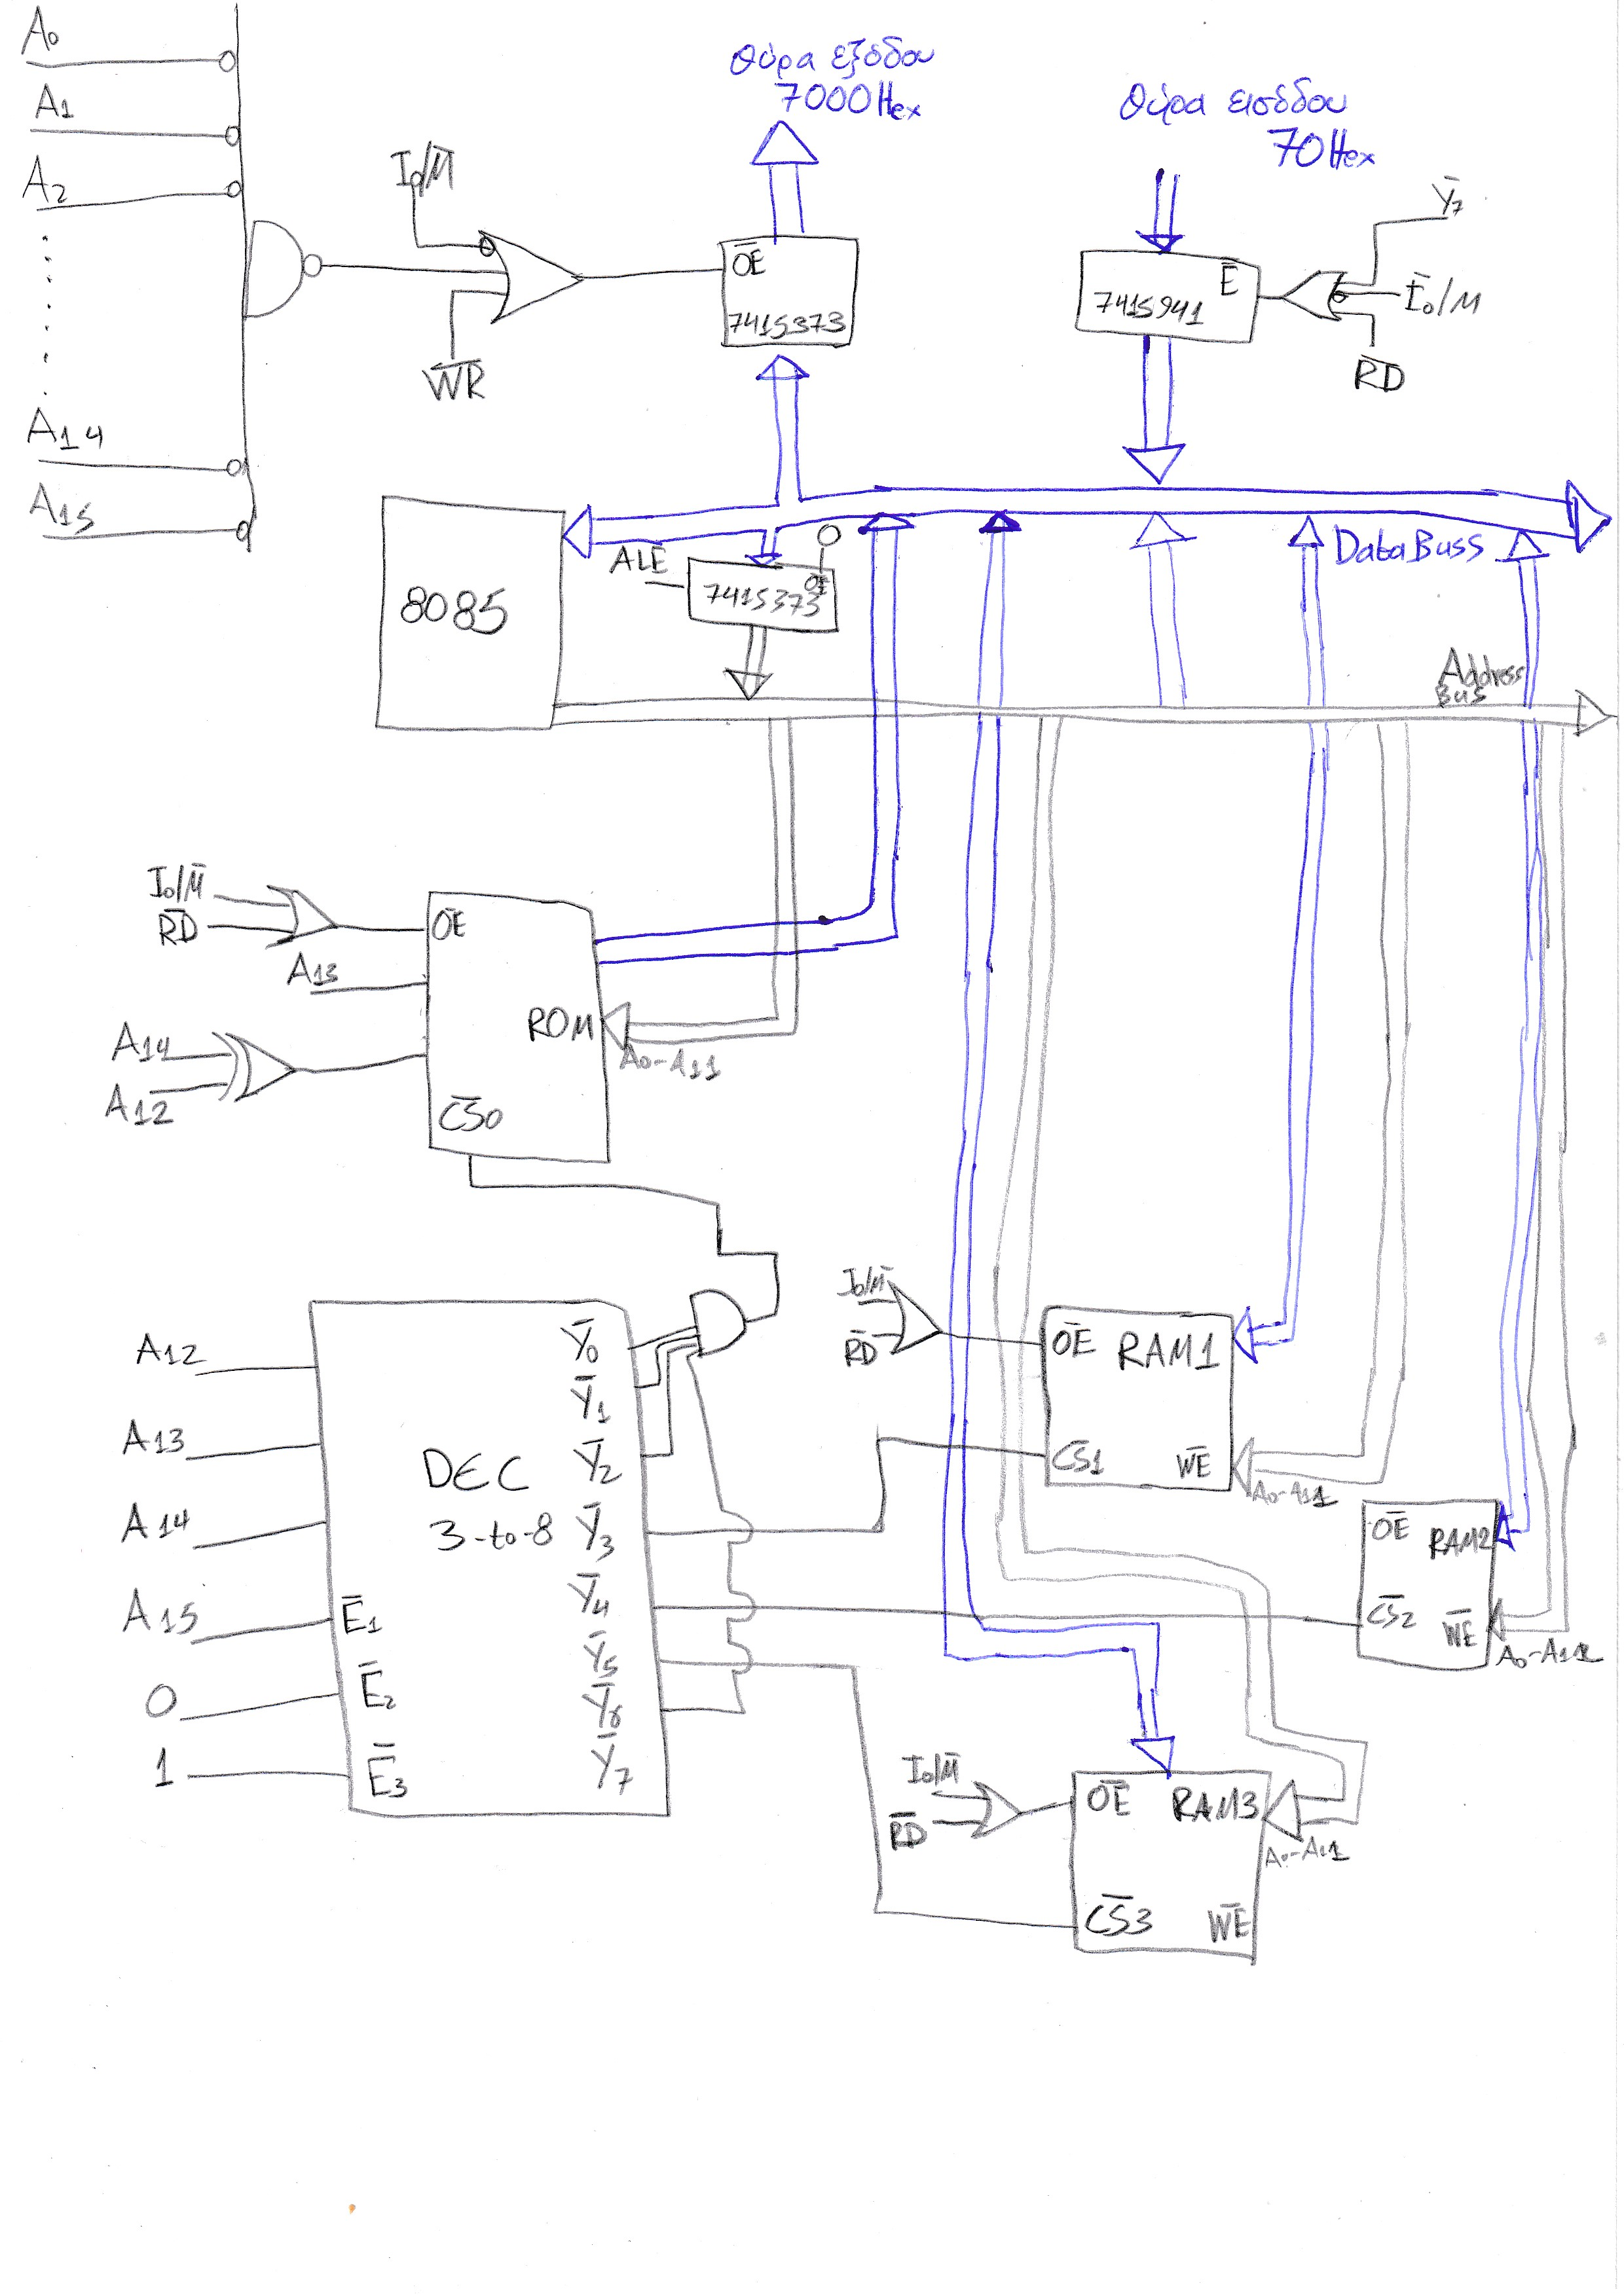
\includegraphics[width=\textwidth]{image2.jpg}
\end{figure}




\end{document}
